\section{Andre Baron}
\label{sec: abaron}

Wzór na deltę: $ \Delta = b^2 - 4ac$
Wzór na pierwiastki równania: \[x=\frac{-b\pm\sqrt{\Delta}}{2a}\]

\begin{figure}[htbp]
    \centering
    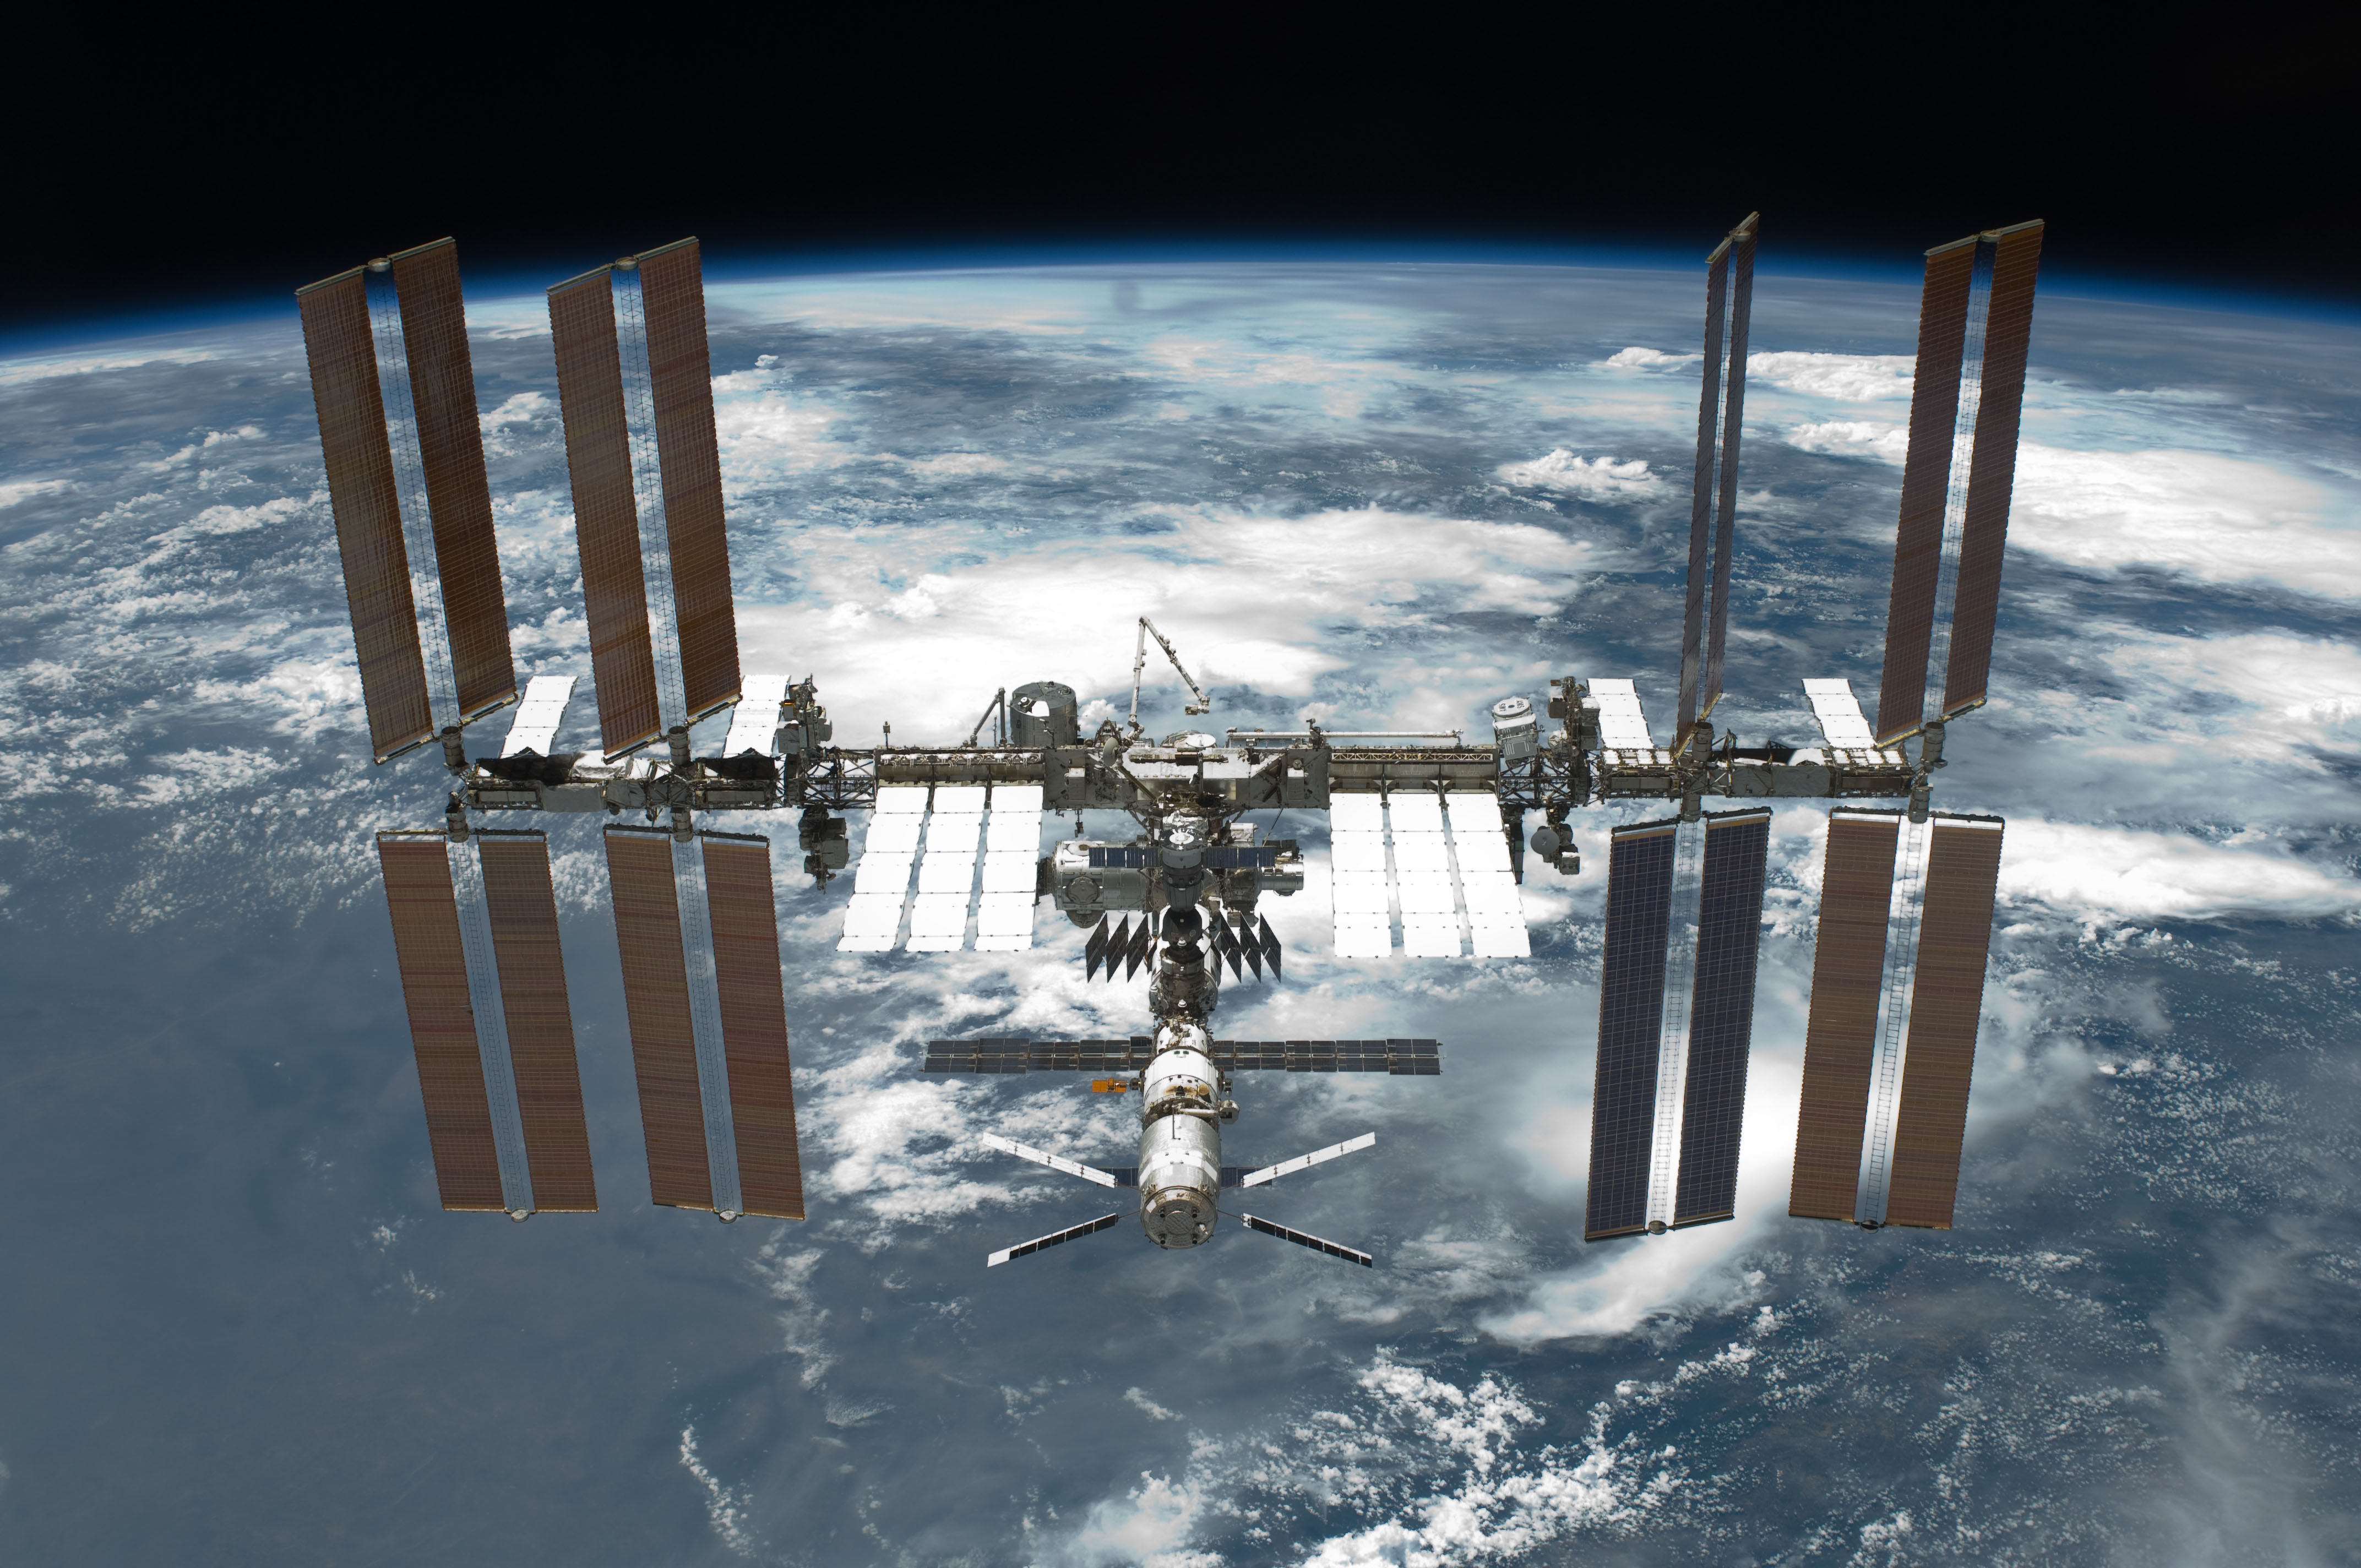
\includegraphics[width=0.7\textwidth]{pictures/iss.jpg}
    \caption{Międzynarodowa stacja kosmiczna}
    \label{fig:iss}
\end{figure}

\begin{enumerate}
    \item Rodzajów statków kosmicznych
    \begin{enumerate}
        \item rakieta
        \item kapsuła
        \item wahadłowiec
        \item samolot kosmiczny
        \item sonda kosmiczna
        \item sztuczny satelita
    \end{enumerate}
\end{enumerate}

\begin{itemize}
    \item Rodzajów statków kosmicznych (ale tym razem nienumerowane)
    \begin{itemize}
        \item rakieta
        \item kapsuła
        \item wahadłowiec
        \item samolot kosmiczny
        \item sonda kosmiczna
        \item sztuczny satelita
    \end{itemize}
\end{itemize}

Zdjęcie stacji kosmicznej~\ref{fig:iss} 

\begin{table}[htbp]
\centering
\begin{tabular}{|l|l|l|l|l|l|}
\hline
liczba płaszczyzn orbitalnych & 72 & 72 & 36 & 6 & 4 \\ \hline
liczba satelitów na płaszczyźnie & 22 & 22 & 20 & 58 & 43 \\ \hline
łączna liczba satelitów & 1584 & 1584 & 720 & 348 & 172  \\ \hline
wysokość & 550 km & 540 km & 570 km & 560 km & 560 km   \\ \hline
inklinacja & $53^\circ$ & $53,2^\circ$ & $70^\circ$ & $97,6^\circ$ & $97,6^\circ$   \\ \hline
\end{tabular}
\label{tab:starlink}
\caption{Orbity satelitów pierwszej części konstelacji Starlink}
\end{table}

Litwo, Ojczyzno moja! ty jesteś jak zdrowie;
Ile cię trzeba cenić, ten tylko się dowie,
Kto cię stracił. Dziś piękność twą w całej ozdobie
Widzę i opisuję, bo tęsknię po tobie.\par

Nam strzelać nie kazano. - \emph{Wstąpiłem na działo}
I spójrzałem na pole; \underline{dwieście armat grzmiało.}
\textbf{Artyleryi ruskiej ciągną się szeregi,}
Prosto, długo, daleko, jako morza brzegi;
\textit{I widziałem ich wodza: przybiegł, mieczem skinął}
I jak ptak jedno skrzydło wojska swego zwinął;
Wylewa się spod skrzydła ściśniona piechota
Długą czarną kolumną, jako lawa błota,
Nasypana iskrami bagnetów. Jak sępy
Czarne chorągwie na śmierć prowadzą zastępy.
\\
\\
Plik został zedytowany lokalnie 09.11.2023 roku pańskiego